\documentclass[]{article}

% Imported Packages
%------------------------------------------------------------------------------
\usepackage{amssymb}
\usepackage{amstext}
\usepackage{amsthm}
\usepackage{amsmath}
\usepackage{enumerate}
\usepackage{fancyhdr}
\usepackage[margin=1in]{geometry}
\usepackage{graphicx}
\usepackage{extarrows}
\usepackage{setspace}
\usepackage{float}
%------------------------------------------------------------------------------

% Header and Footer
%------------------------------------------------------------------------------
\pagestyle{plain}  
\renewcommand\headrulewidth{0.4pt}                                      
\renewcommand\footrulewidth{0.4pt}                                    
%------------------------------------------------------------------------------

% Title Details
%------------------------------------------------------------------------------
\title{Deliverable \#3}
\author{SE 3A04: Software Design II -- Large System Design}
\date{}                               
%------------------------------------------------------------------------------

% Document
%------------------------------------------------------------------------------
\begin{document}

\maketitle	
\noindent{\bf Tutorial Number:} T01\\
{\bf Group Number:} G02 \\
{\bf Group Members:} 
\begin{itemize}
	\item Omer Karo
	\item Ahsan Muzammil
	\item Jake Finlay
	\item Ethan Walsh
	\item Rebecca Di Filippo
	\item Abdallah Alqashqish
\end{itemize}

\newpage

\section{Introduction}
\label{sec:introduction}
% Begin Section

This section should provide an brief overview of the entire document.

\subsection{Purpose}
\label{sub:purpose}
% Begin SubSection
This document provides further information on the architecture of the DealCheck system, including
state chart diagrams, sequence diagrams, and a detailed class diagram.
This document is intended for internal DealCheck stakeholders, including project managers, software developers, domain experts, and members / investors of the DealCheck team. It is recommended that DealCheck deliverables 1 and 2 are read prior to this and the reader has some basic software technical knowledge.
% End SubSection

\subsection{System Description}
\label{sub:system_description}
% Begin SubSection
An overview of the system description and architecture can be found in deliverable 2. This document acts as an extension of deliverable 2, providing more context in the form of detailed diagrams such as state charts, sequence diagrams, and a class diagram.
% End SubSection

\subsection{Overview}
\label{sub:overview}
% Begin SubSection
This document is organized by each individual chart. Section 2 contains state chart diagrams for controller classes, Section 3 contains sequence diagrams, and Section 4 provides a detailed UML class diagram. \newpage
% End SubSection

% End Section

\section{State Charts for Controller Classes}
\label{sec:state_charts_for_controller_classes}
% Begin Section
This section provides a state chart for each controller class for your application.


\begin{figure}[H]
  \centering
  \includegraphics[scale=0.55]{State Diagrams/3A04_state1.png}
  
  \textbf{Figure 2.1:} Account Management Controller State Diagram\label{Fig:2.1}
\end{figure}

\begin{figure}[H]
  \centering
  \includegraphics[scale=0.65]{State Diagrams/3A04_state2.png}
  
  \textbf{Figure 2.2:} Car Recommendation Service Controller State Diagram\label{Fig:2.2}
\end{figure}

\begin{figure}[H]
  \centering
  \includegraphics[scale=0.65]{State Diagrams/3A04_state3.png}
  
  \textbf{Figure 2.3:} Deal Report Management Controller: State Diagram\label{Fig:2.3}
\end{figure}

\begin{figure}[H]
  \centering
  \includegraphics[scale=0.65]{State Diagrams/3A04_state4.png}
  
  \textbf{Figure 2.4:} Experts Process Management Controller: State Diagram\label{Fig:2.4}
\end{figure}

\begin{figure}[H]
  \centering
  \includegraphics[scale=0.65]{State Diagrams/3A04_state5.png}
  
  \textbf{Figure 2.5:} Point System Algorithm Expert Controller: State Diagram\label{Fig:2.5}
\end{figure}

\begin{figure}[H]
  \centering
  \includegraphics[scale=0.65]{State Diagrams/3A04_state6.png}
  
  \textbf{Figure 2.6:} AI Expert Controller: State Diagram\label{Fig:2.6}
\end{figure}

\begin{figure}[H]
  \centering
  \includegraphics[scale=0.65]{State Diagrams/3A04_state7.png}
  
  \textbf{Figure 2.7:} External API Service Expert Controller: State Diagram\label{Fig:2.7}
\end{figure}

\begin{figure}[H]
  \centering
  \includegraphics[scale=0.65]{State Diagrams/3A04_state8.png}
  
  \textbf{Figure 2.8:} Experts Service Controller: State Diagram\label{Fig:2.8}
\end{figure}
% End Section

\section{Sequence Diagrams}
\label{sec:sequence_diagrams}
% Begin Section
This section provides a sequence diagram for each use case of the application.

\begin{figure}[H]
  \centering
  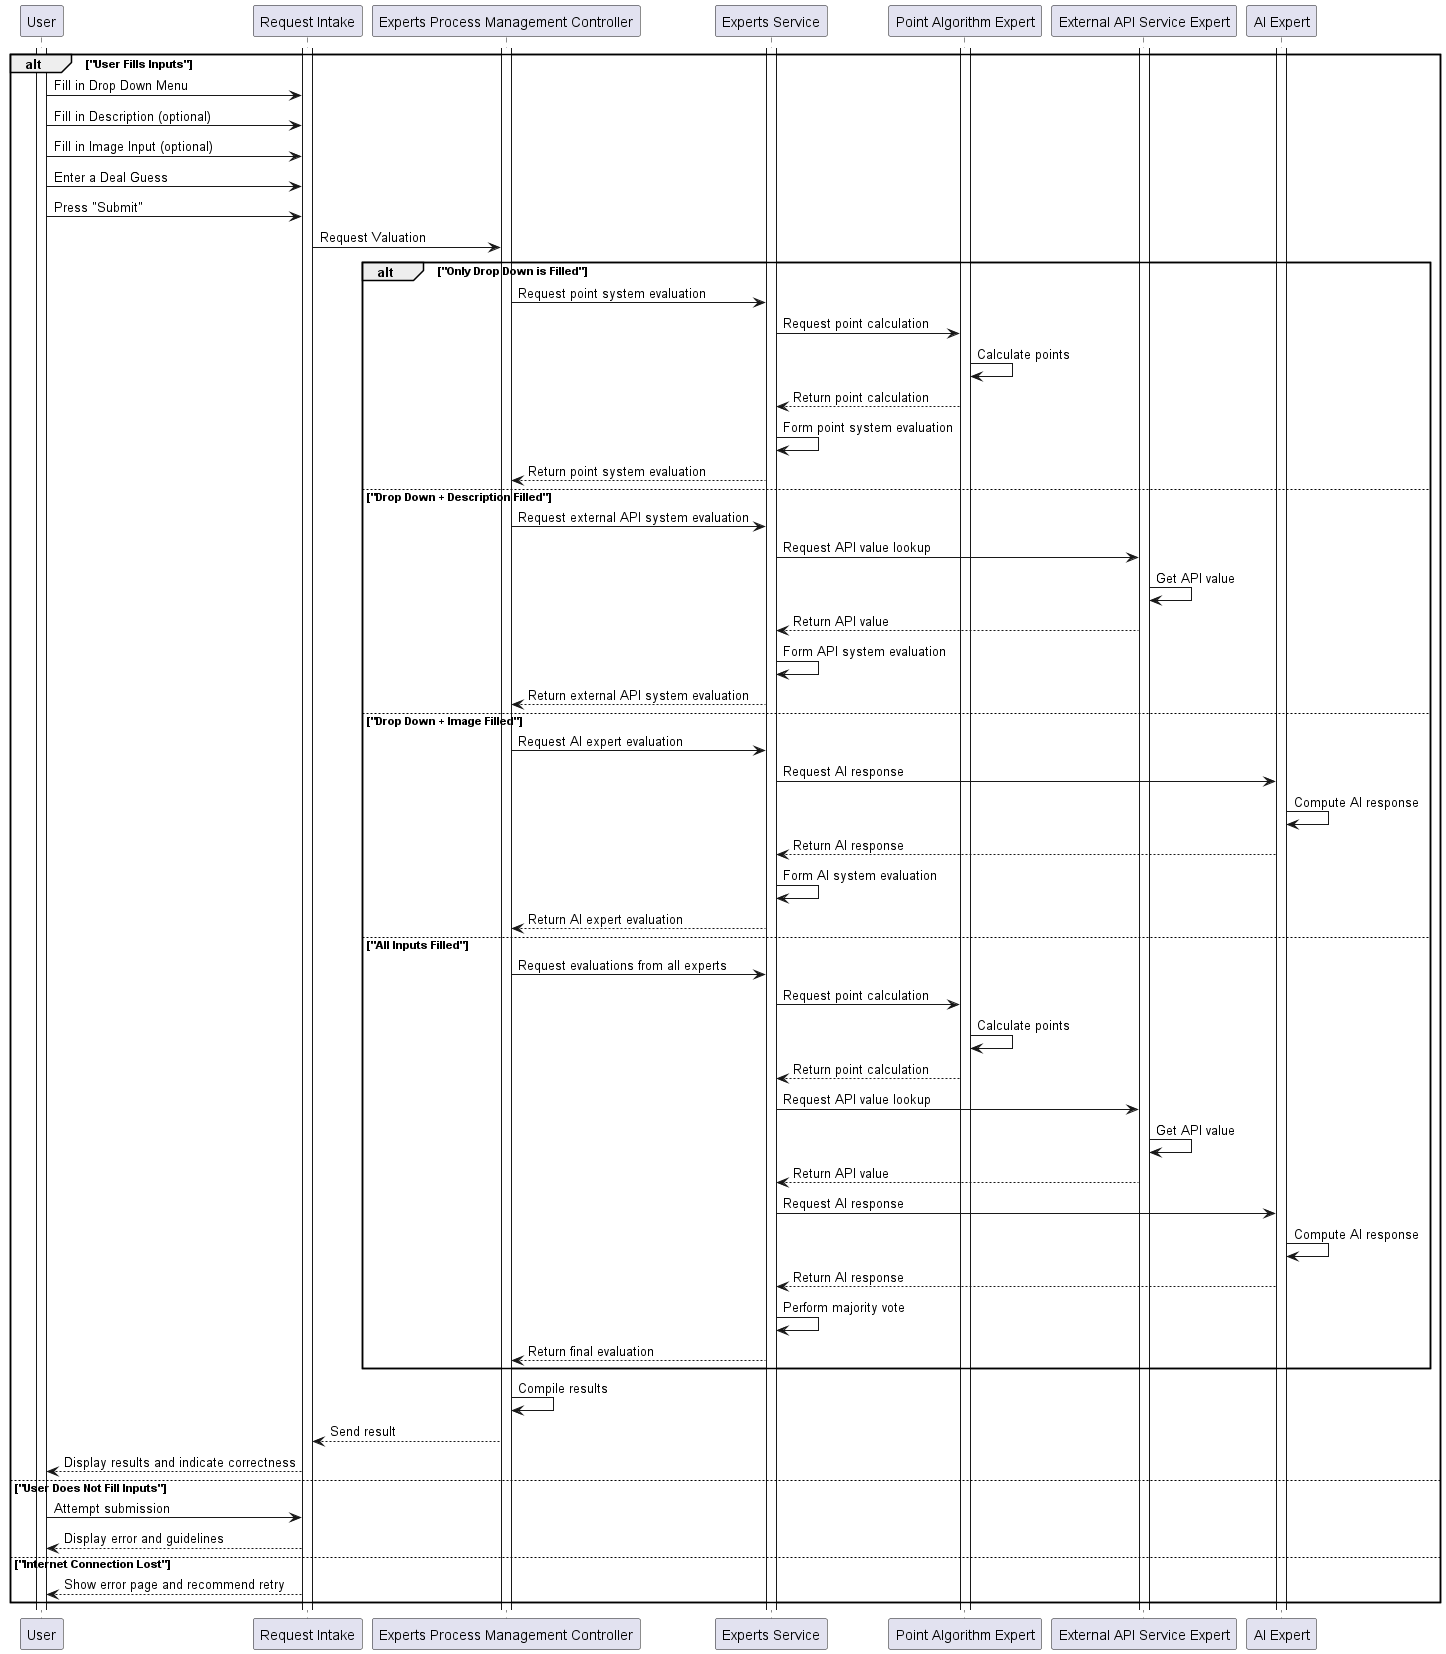
\includegraphics[scale=0.25]{Sequence Diagrams/request.png}
  
  \textbf{Figure 3.1:} Request a Car Deal Valuation: Sequence Diagram\label{Fig:3.1}
\end{figure}

\begin{figure}[H]
  \centering
  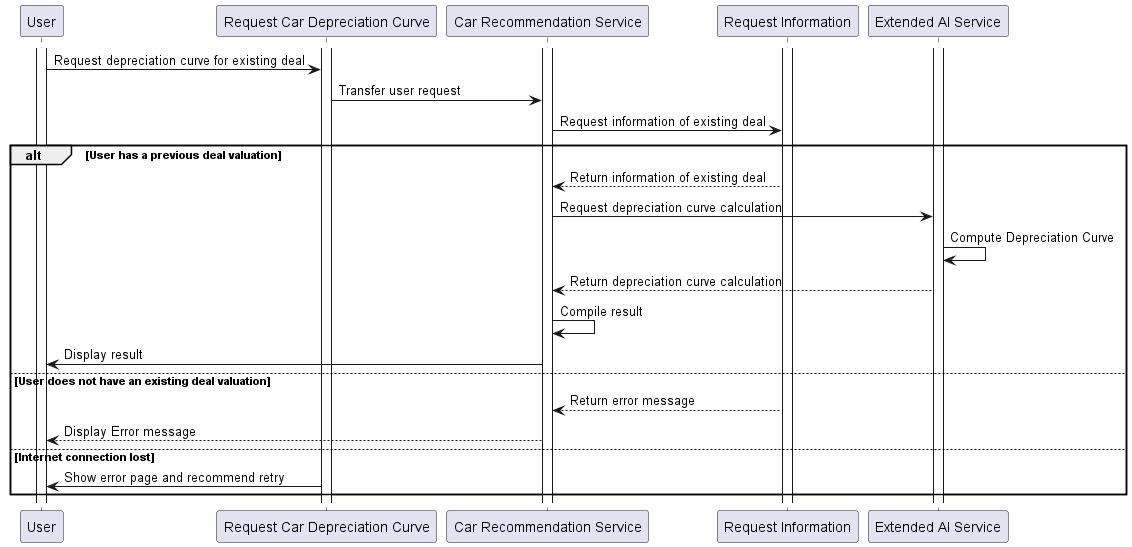
\includegraphics[scale=0.4]{Sequence Diagrams/be4.png}
  
  \textbf{Figure 3.2:} Request a Depreciation Curve: Sequence Diagram\label{Fig:3.2}
\end{figure}

\begin{figure}[H]
  \centering
  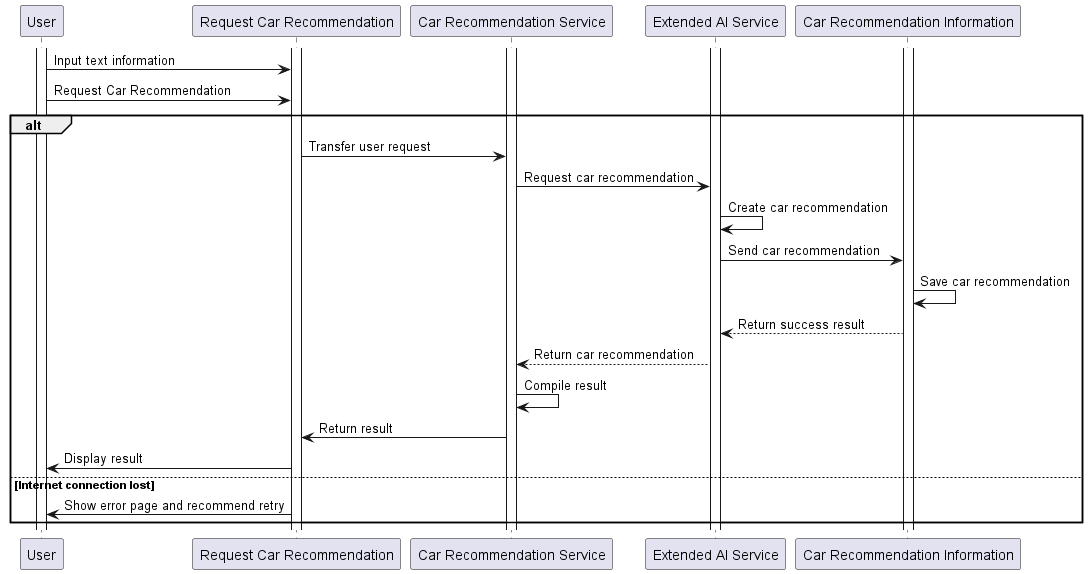
\includegraphics[scale=0.4]{Sequence Diagrams/be6.png}
  
  \textbf{Figure 3.3:} Request a Car Recommendation: Sequence Diagram \label{Fig:3.3}
\end{figure}

\begin{figure}[H]
  \centering
  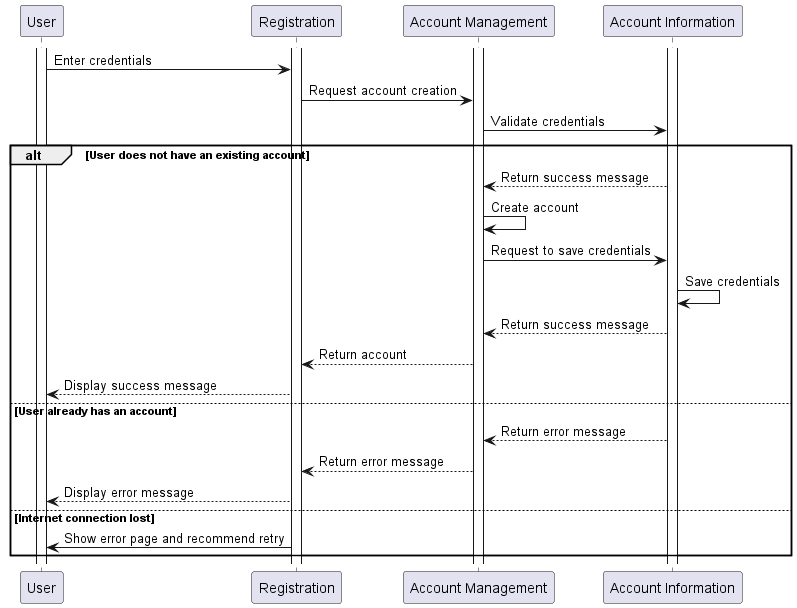
\includegraphics[scale=0.5]{Sequence Diagrams/be8.png}
  
  \textbf{Figure 3.4:} Create Account: Sequence Diagram \label{Fig:3.4}
\end{figure}

\begin{figure}[H]
  \centering
  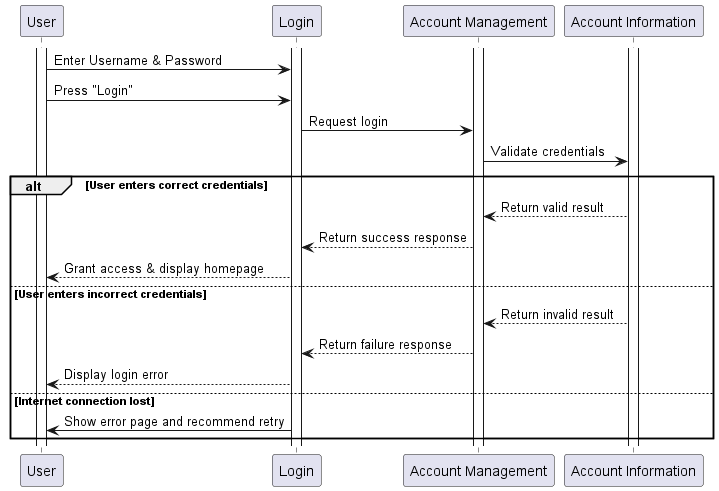
\includegraphics[scale=0.5]{Sequence Diagrams/be9.png}
  
  \textbf{Figure 3.5:} Login: Sequence Diagram\label{Fig:3.5}
\end{figure}

% End Section

\section{Detailed Class Diagram}
\label{sec:detailed_class_diagram}
% Begin Section

\begin{figure}[H]
  \centering
  \includegraphics[scale=0.08]{Class Diagrams/class_diagram_3.jpg}
  
  \textbf{Figure 4.1:} Detailed Class Diagram \label{Fig:4.1}

  Further detail provided in figures 4.1.1 through 4.1.8
\end{figure}

\begin{figure}[H]
  \centering
  \includegraphics[scale=0.04]{Class Diagrams/AccountManagementFeatureSplit.jpg}
  
  \textbf{Figure 4.1.1:} Detailed Class Diagram1 \label{Fig:4.1.1}

  Figure 4.1.1 is the Account Management related classes, found in the center of Figure 4.1.
\end{figure}

\begin{figure}[H]
  \centering
  \includegraphics[scale=0.1]{Class Diagrams/APIFeatureSplit.jpg}
  
  \textbf{Figure 4.1.2:} Detailed Class Diagram2 \label{Fig:4.1.2}

  Figure 4.1.2 is the API Management related classes, found in bottom left of Figure 4.1.
\end{figure}

\begin{figure}[H]
  \centering
  \includegraphics[scale=0.03]{Class Diagrams/CarRecommendationFeatureSplit.jpg}
  
  \textbf{Figure 4.1.3:} Detailed Class Diagram3 \label{Fig:4.1.3}

  Figure 4.1.3 is the Car Recommendation related classes, found on the right of Figure 4.1.
\end{figure}

\begin{figure}[H]
  \centering
  \includegraphics[scale=0.04]{Class Diagrams/DealCheckFeatureSplit.jpg}
  
  \textbf{Figure 4.1.4:} Detailed Class Diagram4 \label{Fig:4.1.4}

  Figure 4.1.4 is the Car Deal Checking related classes, found on the left of Figure 4.1.
\end{figure}


% End Section

\appendix
\section{Division of Labour}
\label{sec:division_of_labour}
% Begin Section
\subsection{Ahsan Muzammil}
\begin{itemize}
  \item Section 4: Created the detailed class diagram for the 2 subsystems of DealCheck.
  \item Section 4: Used draw.io to implement the class diagrams for the Car Recommendation Subsystem and Account Management Subsystem.
  \item Attended Meeting With Abdallah On March 16th to discuss:
        \begin{itemize}
          \item The class diagrams we made
          \item Suggested changes for both of our class diagrams
          \item How to merge the two class diagrams together (Car Recommendation and Account Management with DealCheck feature)
          \item We agreed upon Abdallah merging the two class diagrams into one, using PlantUML
        \end{itemize}
  \item Looked over the merged Class Diagram on PlantUML and suggested some changes to maintain consistency.
        \begin{center}
          
\includegraphics[scale=0.1]{ahsan.jpeg}
        \end{center}
\end{itemize}

\subsection{Rebecca Di Filippo}
\begin{itemize}
   \item Wrote Section 1.1
   \item Wrote Section 1.2
   \item Wrote Section 1.3
    \item Completed 4 state diagrams for controller classes:
        \begin{itemize}
          \item Experts Service Controller
          \item AI Expert Controller
          \item External API Expert Controller 
          \item Point System Algorithm Expert Controller
        \end{itemize}
        \begin{center}
          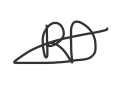
\includegraphics[scale=0.6]{rebecca.png}
        \end{center}
\end{itemize}

\subsection{Ethan Walsh}
\begin{itemize}
  \item Completed 4 state diagrams for controller classes:
        \begin{itemize}
          \item Acount Management Controller
          \item Car Recommendation Service Controller
          \item Deal Report Management
          \item Experts Process Management Controllerr
        \end{itemize}
  \item Proposed edits to other controller class state diagrams.
  \item Performed formatting of diagrams (state, sequence, and class).
  \item Composed and formatted final document in Latex.
  \begin{center}
          
\includegraphics[scale=0.4]{ethan.png}
        \end{center}
\end{itemize}

\subsection{Jake Finlay}
\begin{itemize}
  \item Completed 4 sequence diagrams
        \begin{itemize}
          \item BE1: Request a deal valuation based on drop down menu input
          \item BE3: Request a deal valuation with text description
          \item BE5: Request a deal valuation based on text, drop down, and image input
          \item BE9: Account login
        \end{itemize}
        \begin{center}
          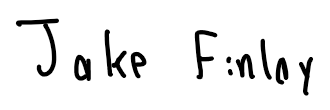
\includegraphics[scale=0.6]{jake.png}
        \end{center}
\end{itemize}

\subsection{Omer Karo}
\begin{itemize}
  \item Completed 4 sequence diagrams
        \begin{itemize}
          \item BE1: Request a deal valuation based on image and required text input
          \item BE3: Request a depreciation curve for a previous car deal report
          \item BE5: Request a car recommendation based on text information provided
          \item BE9: Account creation
        \end{itemize}
        \begin{center}
          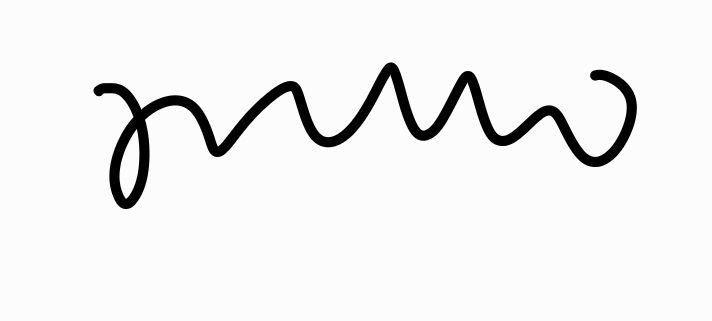
\includegraphics[scale=0.3]{omer.jpg}
        \end{center}
\end{itemize}

\subsection{Abdallah Alqashqish}
\begin{itemize}
  \item Section 4: Created detailed class diagram components for the core DealCheck functionality (checking car deals).
  \item Section 4: Utilized PlantUML to create class diagram for the experts, blackboard, controller of deal checking functionality.
  \item Attended meeting with Ahsan on March 16, 2025 to discuss the following:
    \begin{itemize}
      \item The class diagrams we both made.
      \item Suggested main class architecture styles using interfaces and abstract classes as contracts.
      \item Discussed how to enable the different components of the system to communicate with each other (using router API endpoints).
    \end{itemize}
  \item Merged the two parts of the system into the final class diagram using PlantUML.
  \item Created the split (smaller) class diagrams for each component of the system.
  \item Revised sequence diagrams to ensure consistency with class diagram.
  \begin{center}
    
\includegraphics[scale=0.1]{abdallah.jpg}
  \end{center}
\end{itemize}
% End Section

\newpage
\section*{IMPORTANT NOTES}
\begin{itemize}
	\item You do \underline{NOT} need to provide a text explanation of each diagram; the diagram should speak for itself
	\item Please document any non-standard notations that you may have used
	\begin{itemize}
		\item \emph{Rule of Thumb}: if you feel there is any doubt surrounding the meaning of your notations, document them
	\end{itemize}
	\item Some diagrams may be difficult to fit into one page
	\begin{itemize}
		\item It is OK if the text is small but please ensure that it is readable when printed
		\item If you need to break a diagram onto multiple pages, please adopt a system of doing so and throughly explain how it can be reconnected from one page to the next; if you are unsure about this, please ask me
	\end{itemize}
	\item Please submit the latest version of Deliverable 1 and Deliverable 2 with Deliverable 3
	\begin{itemize}
		\item They do not have to be a freshly printed versions; the latest marked versions are OK
	\end{itemize}
	\item If you do \underline{NOT} have a Division of Labour sheet, your deliverable will \underline{NOT} be marked
\end{itemize}


\end{document}
%------------------------------------------------------------------------------
